\documentclass[journal]{IEEEtran}
% Some very useful LaTeX packages include:
% (uncomment the ones you want to load)


% *** MISC UTILITY PACKAGES ***
%
%\usepackage{ifpdf}
% Heiko Oberdiek's ifpdf.sty is very useful if you need conditional
% compilation based on whether the output is pdf or dvi.
% usage:
% \ifpdf
%   % pdf code
% \else
%   % dvi code
% \fi
% The latest version of ifpdf.sty can be obtained from:
% http://www.ctan.org/pkg/ifpdf
% Also, note that IEEEtran.cls V1.7 and later provides a builtin
% \ifCLASSINFOpdf conditional that works the same way.
% When switching from latex to pdflatex and vice-versa, the compiler may
% have to be run twice to clear warning/error messages.






% *** CITATION PACKAGES ***
%
%\usepackage{cite}
% cite.sty was written by Donald Arseneau
% V1.6 and later of IEEEtran pre-defines the format of the cite.sty package
% \cite{} output to follow that of the IEEE. Loading the cite package will
% result in citation numbers being automatically sorted and properly
% "compressed/ranged". e.g., [1], [9], [2], [7], [5], [6] without using
% cite.sty will become [1], [2], [5]--[7], [9] using cite.sty. cite.sty's
% \cite will automatically add leading space, if needed. Use cite.sty's
% noadjust option (cite.sty V3.8 and later) if you want to turn this off
% such as if a citation ever needs to be enclosed in parenthesis.
% cite.sty is already installed on most LaTeX systems. Be sure and use
% version 5.0 (2009-03-20) and later if using hyperref.sty.
% The latest version can be obtained at:
% http://www.ctan.org/pkg/cite
% The documentation is contained in the cite.sty file itself.






% *** GRAPHICS RELATED PACKAGES ***
%
\ifCLASSINFOpdf
  \usepackage[pdftex]{graphicx}
  % declare the path(s) where your graphic files are
  % \graphicspath{{../pdf/}{../jpeg/}}
  % and their extensions so you won't have to specify these with
  % every instance of \includegraphics
  % \DeclareGraphicsExtensions{.pdf,.jpeg,.png}
\else
  % or other class option (dvipsone, dvipdf, if not using dvips). graphicx
  % will default to the driver specified in the system graphics.cfg if no
  % driver is specified.
  % \usepackage[dvips]{graphicx}
  % declare the path(s) where your graphic files are
  % \graphicspath{{../eps/}}
  % and their extensions so you won't have to specify these with
  % every instance of \includegraphics
  % \DeclareGraphicsExtensions{.eps}
\fi
% graphicx was written by David Carlisle and Sebastian Rahtz. It is
% required if you want graphics, photos, etc. graphicx.sty is already
% installed on most LaTeX systems. The latest version and documentation
% can be obtained at: 
% http://www.ctan.org/pkg/graphicx
% Another good source of documentation is "Using Imported Graphics in
% LaTeX2e" by Keith Reckdahl which can be found at:
% http://www.ctan.org/pkg/epslatex
%
% latex, and pdflatex in dvi mode, support graphics in encapsulated
% postscript (.eps) format. pdflatex in pdf mode supports graphics
% in .pdf, .jpeg, .png and .mps (metapost) formats. Users should ensure
% that all non-photo figures use a vector format (.eps, .pdf, .mps) and
% not a bitmapped formats (.jpeg, .png). The IEEE frowns on bitmapped formats
% which can result in "jaggedy"/blurry rendering of lines and letters as
% well as large increases in file sizes.
%
% You can find documentation about the pdfTeX application at:
% http://www.tug.org/applications/pdftex





% *** MATH PACKAGES ***
%
\usepackage{amsmath}
% A popular package from the American Mathematical Society that provides
% many useful and powerful commands for dealing with mathematics.
%
% Note that the amsmath package sets \interdisplaylinepenalty to 10000
% thus preventing page breaks from occurring within multiline equations. Use:
%\interdisplaylinepenalty=2500
% after loading amsmath to restore such page breaks as IEEEtran.cls normally
% does. amsmath.sty is already installed on most LaTeX systems. The latest
% version and documentation can be obtained at:
% http://www.ctan.org/pkg/amsmath
\usepackage{amssymb}

% *** SPECIALIZED LIST PACKAGES ***
\usepackage{algorithm}
\usepackage{algpseudocode}
% \usepackage{algorithmic}
% algorithmic.sty was written by Peter Williams and Rogerio Brito.
% This package provides an algorithmic environment fo describing algorithms.
% You can use the algorithmic environment in-text or within a figure
% environment to provide for a floating algorithm. Do NOT use the algorithm
% floating environment provided by algorithm.sty (by the same authors) or
% algorithm2e.sty (by Christophe Fiorio) as the IEEE does not use dedicated
% algorithm float types and packages that provide these will not provide
% correct IEEE style captions. The latest version and documentation of
% algorithmic.sty can be obtained at:
% http://www.ctan.org/pkg/algorithms
% Also of interest may be the (relatively newer and more customizable)
% algorithmicx.sty package by Szasz Janos:
% http://www.ctan.org/pkg/algorithmicx


\usepackage{tikz}
\usetikzlibrary{arrows.meta,positioning,fit,calc}

% *** ALIGNMENT PACKAGES ***
%
%\usepackage{array}
% Frank Mittelbach's and David Carlisle's array.sty patches and improves
% the standard LaTeX2e array and tabular environments to provide better
% appearance and additional user controls. As the default LaTeX2e table
% generation code is lacking to the point of almost being broken with
% respect to the quality of the end results, all users are strongly
% advised to use an enhanced (at the very least that provided by array.sty)
% set of table tools. array.sty is already installed on most systems. The
% latest version and documentation can be obtained at:
% http://www.ctan.org/pkg/array


% IEEEtran contains the IEEEeqnarray family of commands that can be used to
% generate multiline equations as well as matrices, tables, etc., of high
% quality.




% *** SUBFIGURE PACKAGES ***
%\ifCLASSOPTIONcompsoc
%  \usepackage[caption=false,font=normalsize,labelfont=sf,textfont=sf]{subfig}
%\else
%  \usepackage[caption=false,font=footnotesize]{subfig}
%\fi
% subfig.sty, written by Steven Douglas Cochran, is the modern replacement
% for subfigure.sty, the latter of which is no longer maintained and is
% incompatible with some LaTeX packages including fixltx2e. However,
% subfig.sty requires and automatically loads Axel Sommerfeldt's caption.sty
% which will override IEEEtran.cls' handling of captions and this will result
% in non-IEEE style figure/table captions. To prevent this problem, be sure
% and invoke subfig.sty's "caption=false" package option (available since
% subfig.sty version 1.3, 2005/06/28) as this is will preserve IEEEtran.cls
% handling of captions.
% Note that the Computer Society format requires a larger sans serif font
% than the serif footnote size font used in traditional IEEE formatting
% and thus the need to invoke different subfig.sty package options depending
% on whether compsoc mode has been enabled.
%
% The latest version and documentation of subfig.sty can be obtained at:
% http://www.ctan.org/pkg/subfig




% *** FLOAT PACKAGES ***
%
%\usepackage{fixltx2e}
% fixltx2e, the successor to the earlier fix2col.sty, was written by
% Frank Mittelbach and David Carlisle. This package corrects a few problems
% in the LaTeX2e kernel, the most notable of which is that in current
% LaTeX2e releases, the ordering of single and double column floats is not
% guaranteed to be preserved. Thus, an unpatched LaTeX2e can allow a
% single column figure to be placed prior to an earlier double column
% figure.
% Be aware that LaTeX2e kernels dated 2015 and later have fixltx2e.sty's
% corrections already built into the system in which case a warning will
% be issued if an attempt is made to load fixltx2e.sty as it is no longer
% needed.
% The latest version and documentation can be found at:
% http://www.ctan.org/pkg/fixltx2e


%\usepackage{stfloats}
% stfloats.sty was written by Sigitas Tolusis. This package gives LaTeX2e
% the ability to do double column floats at the bottom of the page as well
% as the top. (e.g., "\begin{figure*}[!b]" is not normally possible in
% LaTeX2e). It also provides a command:
%\fnbelowfloat
% to enable the placement of footnotes below bottom floats (the standard
% LaTeX2e kernel puts them above bottom floats). This is an invasive package
% which rewrites many portions of the LaTeX2e float routines. It may not work
% with other packages that modify the LaTeX2e float routines. The latest
% version and documentation can be obtained at:
% http://www.ctan.org/pkg/stfloats
% Do not use the stfloats baselinefloat ability as the IEEE does not allow
% \baselineskip to stretch. Authors submitting work to the IEEE should note
% that the IEEE rarely uses double column equations and that authors should try
% to avoid such use. Do not be tempted to use the cuted.sty or midfloat.sty
% packages (also by Sigitas Tolusis) as the IEEE does not format its papers in
% such ways.
% Do not attempt to use stfloats with fixltx2e as they are incompatible.
% Instead, use Morten Hogholm'a dblfloatfix which combines the features
% of both fixltx2e and stfloats:
%
% \usepackage{dblfloatfix}
% The latest version can be found at:
% http://www.ctan.org/pkg/dblfloatfix




%\ifCLASSOPTIONcaptionsoff
%  \usepackage[nomarkers]{endfloat}
% \let\MYoriglatexcaption\caption
% \renewcommand{\caption}[2][\relax]{\MYoriglatexcaption[#2]{#2}}
%\fi
% endfloat.sty was written by James Darrell McCauley, Jeff Goldberg and 
% Axel Sommerfeldt. This package may be useful when used in conjunction with 
% IEEEtran.cls'  captionsoff option. Some IEEE journals/societies require that
% submissions have lists of figures/tables at the end of the paper and that
% figures/tables without any captions are placed on a page by themselves at
% the end of the document. If needed, the draftcls IEEEtran class option or
% \CLASSINPUTbaselinestretch interface can be used to increase the line
% spacing as well. Be sure and use the nomarkers option of endfloat to
% prevent endfloat from "marking" where the figures would have been placed
% in the text. The two hack lines of code above are a slight modification of
% that suggested by in the endfloat docs (section 8.4.1) to ensure that
% the full captions always appear in the list of figures/tables - even if
% the user used the short optional argument of \caption[]{}.
% IEEE papers do not typically make use of \caption[]'s optional argument,
% so this should not be an issue. A similar trick can be used to disable
% captions of packages such as subfig.sty that lack options to turn off
% the subcaptions:
% For subfig.sty:
% \let\MYorigsubfloat\subfloat
% \renewcommand{\subfloat}[2][\relax]{\MYorigsubfloat[]{#2}}
% However, the above trick will not work if both optional arguments of
% the \subfloat command are used. Furthermore, there needs to be a
% description of each subfigure *somewhere* and endfloat does not add
% subfigure captions to its list of figures. Thus, the best approach is to
% avoid the use of subfigure captions (many IEEE journals avoid them anyway)
% and instead reference/explain all the subfigures within the main caption.
% The latest version of endfloat.sty and its documentation can obtained at:
% http://www.ctan.org/pkg/endfloat
%
% The IEEEtran \ifCLASSOPTIONcaptionsoff conditional can also be used
% later in the document, say, to conditionally put the References on a 
% page by themselves.




% *** PDF, URL AND HYPERLINK PACKAGES ***
%
%\usepackage{url}
% url.sty was written by Donald Arseneau. It provides better support for
% handling and breaking URLs. url.sty is already installed on most LaTeX
% systems. The latest version and documentation can be obtained at:
% http://www.ctan.org/pkg/url
% Basically, \url{my_url_here}.




% *** Do not adjust lengths that control margins, column widths, etc. ***
% *** Do not use packages that alter fonts (such as pslatex).         ***
% There should be no need to do such things with IEEEtran.cls V1.6 and later.
% (Unless specifically asked to do so by the journal or conference you plan
% to submit to, of course. )


% correct bad hyphenation here
\hyphenation{op-tical net-works semi-conduc-tor}


\begin{document}
%
% paper title
% Titles are generally capitalized except for words such as a, an, and, as,
% at, but, by, for, in, nor, of, on, or, the, to and up, which are usually
% not capitalized unless they are the first or last word of the title.
% Linebreaks \\ can be used within to get better formatting as desired.
% Do not put math or special symbols in the title.
\title{Receiver-Guided Reinforcement Learning-based Congestion Control for IoT}
%
%
% author names and IEEE memberships
% note positions of commas and nonbreaking spaces ( ~ ) LaTeX will not break
% a structure at a ~ so this keeps an author's name from being broken across
% two lines.
% use \thanks{} to gain access to the first footnote area
% a separate \thanks must be used for each paragraph as LaTeX2e's \thanks
% was not built to handle multiple paragraphs
%

\author{
Qihang~Jiao,~\IEEEmembership{Student Member,~IEEE,}
and~Lotfi~Mhamdi,~\IEEEmembership{Senior Member,~IEEE}%
\thanks{Qihang Jiao and Lotfi Mhamdi are with the School of Electronic and Electrical Engineering, University of Leeds, Leeds, UK (e-mail: el22qj@leeds.ac.uk; L.Mhamdi@leeds.ac.uk).}%
\thanks{Lotfi Mhamdi is also with the College of Computing \& Systems, Abdullah Al Salem University, Kuwait (e-mail: lotfi.mhamdi@aasu.edu.kw).}
}
%                     ^------------^------------^----Do not want these spaces!
%
% a space would be appended to the last name and could cause every name on that
% line to be shifted left slightly. This is one of those "LaTeX things". For
% instance, "\textbf{A} \textbf{B}" will typeset as "A B" not "AB". To get
% "AB" then you have to do: "\textbf{A}\textbf{B}"
% \thanks is no different in this regard, so shield the last } of each \thanks
% that ends a line with a % and do not let a space in before the next \thanks.
% Spaces after \IEEEmembership other than the last one are OK (and needed) as
% you are supposed to have spaces between the names. For what it is worth,
% this is a minor point as most people would not even notice if the said evil
% space somehow managed to creep in.



% The paper headers
% \markboth{Journal of \LaTeX\ Class Files,~Vol.~14, No.~8, August~2015}%
% {Shell \MakeLowercase{\textit{et al.}}: Bare Demo of IEEEtran.cls for IEEE Journals}
% The only time the second header will appear is for the odd numbered pages
% after the title page when using the twoside option.
% 
% *** Note that you probably will NOT want to include the author's ***
% *** name in the headers of peer review papers.                   ***
% You can use \ifCLASSOPTIONpeerreview for conditional compilation here if
% you desire.




% If you want to put a publisher's ID mark on the page you can do it like
% this:
%\IEEEpubid{0000--0000/00\$00.00~\copyright~2015 IEEE}
% Remember, if you use this you must call \IEEEpubidadjcol in the second
% column for its text to clear the IEEEpubid mark.



% use for special paper notices
%\IEEEspecialpapernotice{(Invited Paper)}




% make the title area
\maketitle

% As a general rule, do not put math, special symbols or citations
% in the abstract or keywords.
\begin{abstract}
The abstract goes here.
\end{abstract}

% Note that keywords are not normally used for peerreview papers.
\begin{IEEEkeywords}
IoT, TCP, congestion control, reinforcement learning.
\end{IEEEkeywords}






% For peer review papers, you can put extra information on the cover
% page as needed:
% \ifCLASSOPTIONpeerreview
% \begin{center} \bfseries EDICS Category: 3-BBND \end{center}
% \fi
%
% For peerreview papers, this IEEEtran command inserts a page break and
% creates the second title. It will be ignored for other modes.
\IEEEpeerreviewmaketitle

\section{Introduction}
% The very first letter is a 2 line initial drop letter followed
% by the rest of the first word in caps.
% 
% form to use if the first word consists of a single letter:
% \IEEEPARstart{A}{demo} file is ....
% 
% form to use if you need the single drop letter followed by
% normal text (unknown if ever used by the IEEE):
% \IEEEPARstart{A}{}demo file is ....
% 
% Some journals put the first two words in caps:
% \IEEEPARstart{T}{his demo} file is ....
% 
% Here we have the typical use of a "T" for an initial drop letter
% and "HIS" in caps to complete the first word.
% \IEEEPARstart{T}{his} demo file is intended to serve as a ``starter file''
% for IEEE journal papers produced under \LaTeX\ using
% IEEEtran.cls version 1.8b and later.
% % You must have at least 2 lines in the paragraph with the drop letter
% % (should never be an issue)
% I wish you the best of success.
\IEEEPARstart{T}{his} part is to be completed.

\section{Related Works}
This part is to be completed.

\begin{figure}[h]
\centering
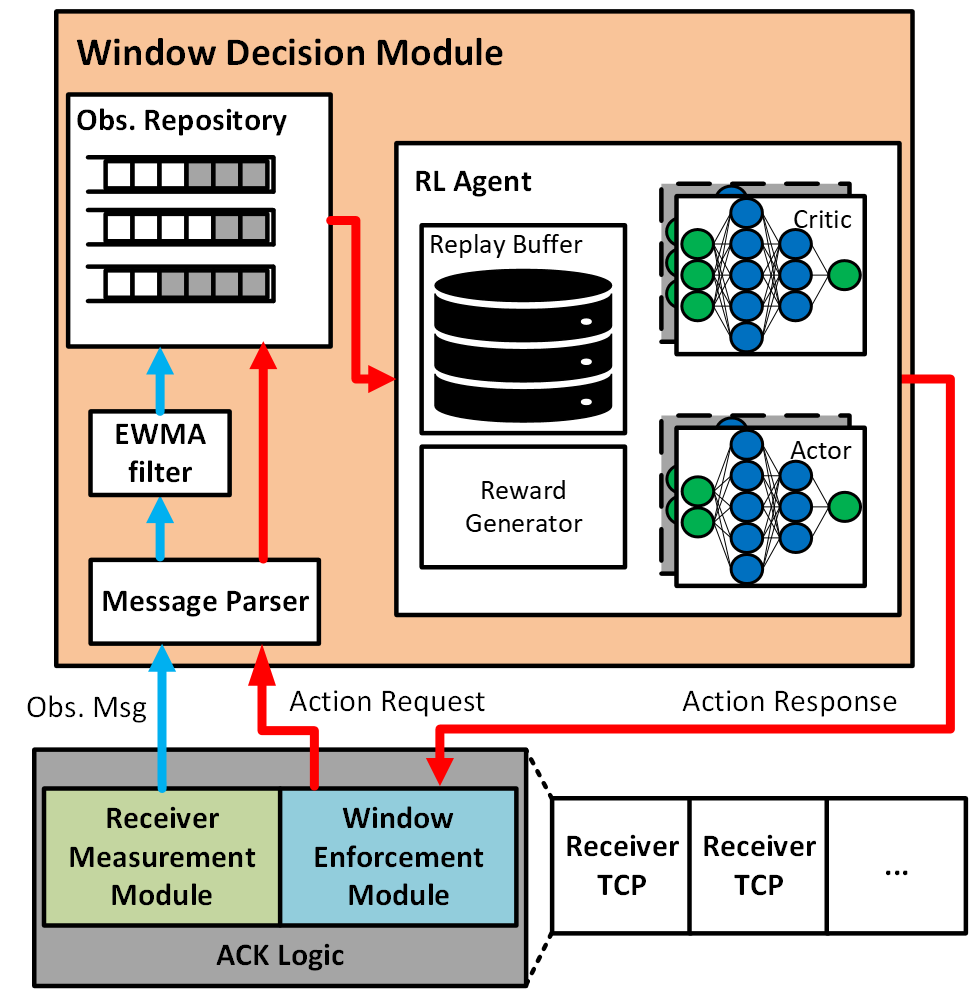
\includegraphics[width=0.95\linewidth]{./fig/SystemArchitecture2_7.png}
\caption{System architecture of our proposal.}
\label{SysArch}
\end{figure}

\section{System Design}
Our proposal contains three modules in the receiver side for adjusting sender $cwnd$, Receiver Measurement Module, Window Decision Module, and Window Enforcement Module.
For better compatibility of our design, TCP sockets in both sender and receiver are extended or modified for adding interfaces and able to send three control messages to achieved our features.

\subsection{Control Message types definition}
% The receiver TCP socket is extended to have features to communicate with our agent. We defined messages into three types 'state', 'action request', 'connection close' for agent to execute either store the states into its replay buffer, output an action, or clear the states for the closed connection.

The receiver TCP socket is extended to support communication with the RL agent. 
Three types of messages are defined:

\begin{itemize}
    \item \textbf{Observation Message}: carries the observed network status and is sent to the agent for storage in the replay buffer.
    
    \item \textbf{Action Request}: triggers the agent to infer and return a control action based on the current state.
    
    \item \textbf{Connection Close}: notifies the agent that a flow has terminated, allowing it to clear the corresponding internal states.
\end{itemize}

\subsection{Receiver Measurement Module}
Our scheme relies on reliable state observations to ensure stable training. Therefore, the states in our design are required to reflect the congestion extent while remaining observable at the receiver. Despite RTT is a fine-grained and valuable indicator of congestion, it is difficult to directly observe in the receiver side.

To address the limitation above, we derive a receiver-side congestion extent metric based on the $cwnd$ elapsed time ($t_{elapsed}$). We extend the sender TCP feature to include its $cwnd$ in TCP header. 
In standard TCP congestion avoidance, the congestion window $cwnd$ is increased by 1 MSS after an entire $cwnd$ bytes has been acknowledged. This nature results in an approximate growth rate of 1 MSS per RTT, in which the method is named Additive Increment.

We utilise Additive Increment growing feature to enable the receiver to estimate network congestion extent by calculating the elapsed time for a flow to complete its $cwnd$.
In particular, upon every packet receive event that includes a $cwnd$ value different from the last value received, the Receiver Measurement Module establishes a new estimation task.

\begin{figure}[!t]
\centering
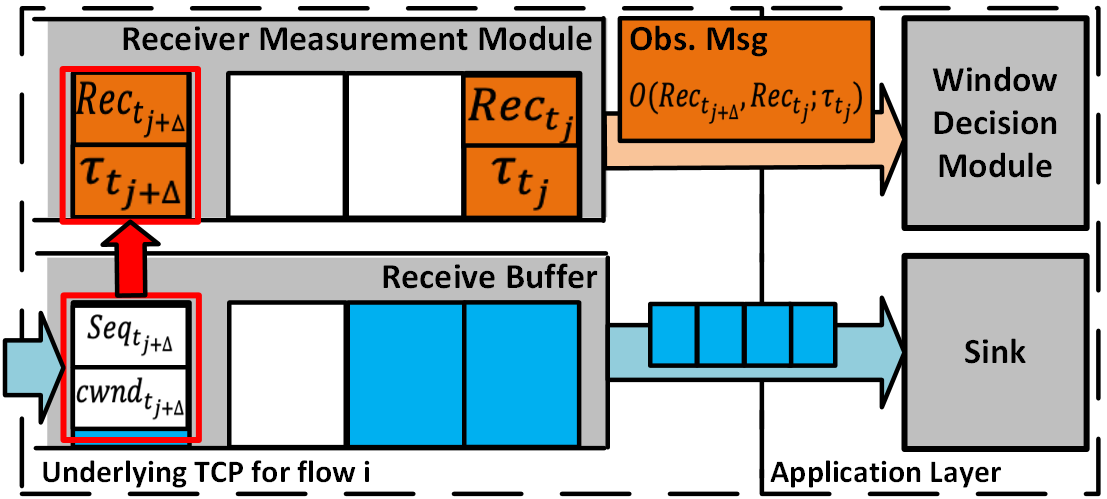
\includegraphics[width=\linewidth]{./fig/ReceiverMeasurementModule3.png}
\caption{An example of estimation task completion of flow $i$.}
\label{Estimation}
\end{figure}

A new task is initialised with a record ($Rec$) for the current flow state and a threshold ($\tau$), e.g., for flow $i$ started at time $t_0$ and estimated at time $t_j$, defined as below:
\begin{equation}
  Rec_{i,t_j}\triangleq[B_i(t_j), L_i(t_j), t_j]
\end{equation} 
where we set $\tau$ to be the sum of sequence number ($Seq_{i,t_j}$) and the $cwnd$ value from its header. We also maintain a cumulative received bytes ($RxBytes_{i,t}$) and cumulative packet losses ($Losses_{i,t}$) counter in the receiver TCP, defined as follows:
\begin{equation}
  \tau_{i,t_j} = Seq_{i, t_j} + cwnd_{i,t_j}
\end{equation}
\begin{equation}
  B_i(t_j) = \sum_{n = t_0}^{t_j} Rx Bytes_{i, n}
\end{equation} 
\begin{equation}
  L_i(t_j) = \sum_{n= t_0}^{t_j}Losses_{i, n}
\end{equation} 

An estimation task is completed at $t_{j+\Delta}$ when a coming packet is seen with a sequence number satisfying $Seq_{i,t_{j+\Delta}} > \tau_{i,t_j}$.
We calculate this task duration as the $cwnd$ elapsed time i.e., $t_{elapsed} = t_{j+\Delta} - t_{j}$. We then calculate the goodput ($g_{i, t_j}$) and packet losses during the estimation task, where $g_{i, t_j} = \frac{B_i(t_{j+\Delta})-B_i(t_j)}{t_{elapsed}}$. and $\ell_{i,t_j} = L_i(t_{j+\Delta})-L_i(t_j)$. Therefore, an observation is formed denoted as 
$o_{i,t_j}=O(Rec_{i,t_{j+\Delta}},Rec_{i,t_{j}};\tau_{i,t_j})$, with the observation as the result of the generation process defined as follows:
$$ O(Rec_{i,t_{j+\Delta}},Rec_{i,t_{j}};\tau_{i,t_j}) \triangleq \left[g_{i, t_j}, \ell_{i,t_j}, t_{elapsed}\right]$$
The eventual observation is encapsulated into a Observation Message and sent to the Window Decision Module for storage. The consecutive process triggered by packet received event can be seen in Algorithm~\ref{alg:per_packet_state}.

\begin{algorithm}[t]
\renewcommand{\algorithmicrequire}{\textbf{Input:}}
\renewcommand{\algorithmicensure}{\textbf{Output:}}
\caption{Receiver Measurement and Observation Generation}
\label{alg:per_packet_state}
\begin{algorithmic}[1]
\Require Flow Id $i$, Time $t_j$, Arrived Packet $p_{i,t_j}$, Flow Observation Queue $q_i$
\Ensure Observation $o_{i,t_j}$, Control Message $M$
\State Extract $Seq_{i,t_j}$, $cwnd_{i,t_j}$, and $RxBytes_{i,t_j}$ from $p_{i,t_j}$
\State $\tau_{i,t_j} = Seq_{i,t_j}+cwnd_{i,t_j}$
\State Obtain $Losses_{i,t_j}$ from $TcpSocket_i$
\State $B_i(t_j) = B_i(t_{j-1})+ Rx Bytes_{i, t_j}$
\State $L_i(t_j) = L_i(t_{j-1}) + Losses_{i,t_j}$
\State $Rec_{i,t_j}=\left[B_i(t_j), L_i(t_j), t_j\right]$
\State Obtain $Rec_{i}^{head}$ and $\tau_{i}^{head}$ from the head of $q_i$
\If{$Seq_{i,t_j} \ge \tau_{i}^{head}$}
  \State Dequeue $Rec_{i}^{head}$ and $\tau_{i}^{head}$ from $q_i$
  \State $o_{i,t_{j}} = O(Rec_{i,t_j},Rec_{i}^{head})$
  % \State Send $o_{i,t_{j}}$ included into State Message to Agent
  \State Include $o_{i,t_{j}}$ into $M$
  \State Send $M$ to agent
\ElsIf{$cwnd_{i,t_j} \neq cwnd_{i,t_{j-1}}$}
  \State Enqueue $Rec_{i,t_j}$ and $\tau_{i,t_j}$ into $q_i$
\EndIf
\end{algorithmic}
\end{algorithm}

\begin{algorithm}[t]
\renewcommand{\algorithmicrequire}{\textbf{Input:}}
\renewcommand{\algorithmicensure}{\textbf{Output:}}
\caption{Window Decision Module}
\label{alg:window_decision_module}
\begin{algorithmic}[1]
\Require Control Message $M$, Replay Buffer $B$, Flow State Buffer $B_i$ for flow $i$, Batch Size $N$
\Ensure 
\If{$M$ = "Connnection Close"}
\State Clear $B_i$
\ElsIf{$M$ = "State"}
\State Extract $s_i$ from $M$
\State Store $s_i$ into $B_i$
\ElsIf{$M$ = "Action Request"}
\State Compute the average state $\bar{s_i}$ over $B_i$
\State $a = \mu(\bar{s_i};\theta^{\mu})$
\State Store transition $(\bar{s_i}, a_i, r_i, \bar{s_{i}}^{'})$ into $B$
\State Randomly sample $N$ transition from $B$
\State Compute $y_t=r(s_t,a_t)+\gamma Q^{-}(s_{t+1},\mu^{-}(s_{t+1}))$
\State Compute $L(\theta^Q) = \mathbb{E}[(Q(s_t,a_t;\theta^{Q}) - y_t)^2]$
\State Update Critic minimising $L(\theta^Q)$
\State Compute $\nabla_{\theta^\mu} J(\theta^\mu) = \mathbb{E}[\nabla_{a_t}Q(s_t,\mu(s_t))
\nabla_{\theta^\mu} \mu(s_t)]$
\State Update Actor via gradient ascent $\nabla_{\theta^\mu} J(\theta^\mu)$
\State $\theta^{\mu^-} \leftarrow \tau \times \theta + (1-\tau)\times \theta^{\mu^-}$
\State $\theta^{Q^-} \leftarrow \tau \times \theta + (1-\tau)\times \theta^{Q^-}$
\EndIf
\end{algorithmic}
\end{algorithm}

\subsection{Window Decision Module}
% action_block 这里写，算了，写agent吧
Window Decision Module consists of a Reinforcement Learning model to output a scaling factor to underlying TCP socket periodically triggered by Action Request from Window Enforcement Module.
An enforced congestion window is then calculated with the factor by the underlying TCP socket and included in ACK to the sender. The sender will overwrite its $cwnd$ by the enforced congestion window. Therefore, to implement a continuous control to modified TCP, we choose Deep Deterministic Policy Gradient (DDPG) as agent in our design.

\subsubsection{State Generation}

\subsubsection{Reward Design}

\subsubsection{Training}
Our agent consists of an actor network determining a deterministic action $a = \mu(s;\theta^{\mu})$ parameterised by $\theta^{\mu}$ and a critic network to approximate the expected future return, defined as $Q(s,a;\theta^{Q}) = \mathbb{E}[R_t|s_t,a_t]$ with parameters $\theta^{Q}$. 
The return $R_t$ is the sum of discounted future return, i.e., $R_t = \sum_{i=t}^{T}\gamma^{i-t}r(s_i,a_i)$. Approaching to the approximation is done by updating the critic network through minimising the mean square error between its output and a target function ($y_t$), shown as follows:
$$ L(\theta^Q) = \mathbb{E}[(Q(s_t,a_t;\theta^{Q}) - y_t)^2] $$
$$y_t=r(s_t,a_t) + \gamma Q^{-}(s_{t+1}, \mu^{-}(s_{t+1};\theta^{\mu^-});\theta^{Q^-})$$ 
where $Q^{-}(s, a;\theta^{-})$ and $\mu^{-}(s;\theta^{\mu^-})$ are target critic network and target policy network. Their parameters are updated by calculating the exponetially weighted moving average of critic network and policy network, i.e., $\theta^{-} \leftarrow \tau \times \theta + (1-\tau)\times \theta^{-}$ where the $\tau$ is the weight parameter.
Subsequently, with the updated critic network, policy performance of current actor network is predicted, expressed as $J(\theta^\mu) = \mathbb{E}[Q(s_t,\mu(s_t;\theta^\mu))]$.
Training an actor network is done by updating its paramters through policy performance gradient ascent. Specifically, by applying the chain rule, the gradient of the policy performance, is computed as:
$$\nabla_{\theta^\mu} J(\theta^\mu) = \mathbb{E}[\nabla_{a_t}Q(s_t,\mu(s_t;\theta^\mu))
\nabla_{\theta^\mu} \mu(s_t;\theta^\mu)]$$

\subsection{Window Enforcement Module}
For an RL-controlled CC, it is important that waiting agent for action generation should not block the TCP normal behaviour. Therefore, we decouple the Window Decision Module, Receiver Measurement Module and standard feature to ensure none of them will block any other. Therefore, an ACK response will not be delayed due to our scheme. 
In our design, an action request message will be sent to agent periodically by Window Decision Module. The resulting action is a factor within $[0,1]$. Once the Window Decision Module receive the action, it will extract the latest $cwnd$ in Receiver Measurement Module and compute the enforced congestion window using the following:
$$cwnd_{enforced} = cwnd \times scaling\_factor ^ {a},\ n \in[0,1]$$
Then the enforced $cwnd$ will be included into the ACK header and take effect at the sender side. For the receiver, the same action will keep effective untill the next action request.


\section{Simulation setup and results}


% An example of a floating table. Note that, for IEEE style tables, the
% \caption command should come BEFORE the table and, given that table
% captions serve much like titles, are usually capitalized except for words
% such as a, an, and, as, at, but, by, for, in, nor, of, on, or, the, to
% and up, which are usually not capitalized unless they are the first or
% last word of the caption. Table text will default to \footnotesize as
% the IEEE normally uses this smaller font for tables.
% The \label must come after \caption as always.
%
%\begin{table}[!t]
%% increase table row spacing, adjust to taste
%\renewcommand{\arraystretch}{1.3}
% if using array.sty, it might be a good idea to tweak the value of
% \extrarowheight as needed to properly center the text within the cells
%\caption{An Example of a Table}
%\label{table_example}
%\centering
%% Some packages, such as MDW tools, offer better commands for making tables
%% than the plain LaTeX2e tabular which is used here.
%\begin{tabular}{|c||c|}
%\hline
%One & Two\\
%\hline
%Three & Four\\
%\hline
%\end{tabular}
%\end{table}


% Note that the IEEE does not put floats in the very first column
% - or typically anywhere on the first page for that matter. Also,
% in-text middle ("here") positioning is typically not used, but it
% is allowed and encouraged for Computer Society conferences (but
% not Computer Society journals). Most IEEE journals/conferences use
% top floats exclusively. 
% Note that, LaTeX2e, unlike IEEE journals/conferences, places
% footnotes above bottom floats. This can be corrected via the
% \fnbelowfloat command of the stfloats package.




\section{Conclusion}
The conclusion goes here.





% if have a single appendix:
%\appendix[Proof of the Zonklar Equations]
% or
%\appendix  % for no appendix heading
% do not use \section anymore after \appendix, only \section*
% is possibly needed

% use appendices with more than one appendix
% then use \section to start each appendix
% you must declare a \section before using any
% \subsection or using \label (\appendices by itself
% starts a section numbered zero.)
%


% \appendices
% \section{Proof of the First Zonklar Equation}
% Appendix one text goes here.

% % you can choose not to have a title for an appendix
% % if you want by leaving the argument blank
% \section{}
% Appendix two text goes here.


% use section* for acknowledgment
\section*{Acknowledgment}


The authors would like to thank...


% Can use something like this to put references on a page
% by themselves when using endfloat and the captionsoff option.
\ifCLASSOPTIONcaptionsoff
  \newpage
\fi



% trigger a \newpage just before the given reference
% number - used to balance the columns on the last page
% adjust value as needed - may need to be readjusted if
% the document is modified later
%\IEEEtriggeratref{8}
% The "triggered" command can be changed if desired:
%\IEEEtriggercmd{\enlargethispage{-5in}}

% references section

% can use a bibliography generated by BibTeX as a .bbl file
% BibTeX documentation can be easily obtained at:
% http://mirror.ctan.org/biblio/bibtex/contrib/doc/
% The IEEEtran BibTeX style support page is at:
% http://www.michaelshell.org/tex/ieeetran/bibtex/
%\bibliographystyle{IEEEtran}
% argument is your BibTeX string definitions and bibliography database(s)
%\bibliography{IEEEabrv,../bib/paper}
%
% <OR> manually copy in the resultant .bbl file
% set second argument of \begin to the number of references
% (used to reserve space for the reference number labels box)
\begin{thebibliography}{1}

\bibitem{IEEEhowto:kopka}
H.~Kopka and P.~W. Daly, \emph{A Guide to \LaTeX}, 3rd~ed.\hskip 1em plus
  0.5em minus 0.4em\relax Harlow, England: Addison-Wesley, 1999.

\end{thebibliography}

% biography section
% 
% If you have an EPS/PDF photo (graphicx package needed) extra braces are
% needed around the contents of the optional argument to biography to prevent
% the LaTeX parser from getting confused when it sees the complicated
% \includegraphics command within an optional argument. (You could create
% your own custom macro containing the \includegraphics command to make things
% simpler here.)
%\begin{IEEEbiography}[{\includegraphics[width=1in,height=1.25in,clip,keepaspectratio]{mshell}}]{Michael Shell}
% or if you just want to reserve a space for a photo:

% \begin{IEEEbiography}{Michael Shell}
% Biography text here.
% \end{IEEEbiography}

% % if you will not have a photo at all:
% \begin{IEEEbiographynophoto}{John Doe}
% Biography text here.
% \end{IEEEbiographynophoto}

% insert where needed to balance the two columns on the last page with
% biographies
%\newpage

% \begin{IEEEbiographynophoto}{Jane Doe}
% Biography text here.
% \end{IEEEbiographynophoto}

% You can push biographies down or up by placing
% a \vfill before or after them. The appropriate
% use of \vfill depends on what kind of text is
% on the last page and whether or not the columns
% are being equalized.

%\vfill

% Can be used to pull up biographies so that the bottom of the last one
% is flush with the other column.
%\enlargethispage{-5in}



% that's all folks
\end{document}


